\documentclass[a4paper,12pt]{llncs}
\usepackage[top=75pt, bottom=75pt, left=85pt, right=85pt]{geometry}

\usepackage{amssymb}
\setcounter{tocdepth}{3}
\usepackage{graphicx}
\usepackage{soul,color}
\usepackage{url}
\usepackage{algorithm}
%\usepackage{enumitem}
\newcommand{\keywords}[1]{\par\addvspace\baselineskip
\noindent\keywordname\enspace\ignorespaces#1}
\newcommand{\ie}{i.e.} 
\newcommand{\eg}{e.g.} 
\newcommand{\et}{et al. }

\begin{document}
\title{Weekly Report -- 49}
\author{Xiufeng Liu}
\institute{University of Waterloo, CA\\
\email{xiufeng.liu@uwaterloo.ca}
}
\maketitle


\section{This Week}
This week I first investigate the benchmark study for energy data analysis. Inspired by the IBM technical report \cite{ibmbenchmark}, I outlined the benchmark process in Section~\ref{sec:benchmark}. The process basically follows the route as the IBM benchmark, \texttt{data validation (cleansing)$\Rightarrow$ data loading $\Rightarrow$ analysis}. But, according to our discussion on Wednesday, our benchmark experiments will not totally follow this route. Instead, we could benchmark the analysis for electricity data with different technologies combinations. 

The other work of this week is re-exported the ESSEX data sets with timestamp attribute.

\section{Next Week}
The work of next week will focus on the study of the use of SciDB and KDB. This includes the data models design, importing the data, and re-write analysis algorithms using q language for KDB, R language for SciDB, etc.

\subsection{The Process of Benchmark Study}
\label{sec:benchmark}
\paragraph{Benchmark of Data Cleansing and Loading Process:} 
Metering data is corrected from innumerable meters and sensors deployed at different locations. The meter readings and  sensor data are collected at pre-defined time interval.  An important fact is that the meter and sensor data are not always collect, and consistent. For example,  a defected meter could produce abnormal data, a meter stopped working will cause data missing, and changing of a new meter with a different unit will cause the  inconsistency of the readings. Therefore, an important part of the data analysis process is to access the quality of the data, and  consider to ``modifying" them in order to improve the quality of the analysis results, e.g, by removing any obvious errors. This process is often called {\em data cleansing}, which is an essential precursor to attempting to model data. The data cleansing process might include identifying and removing the obvious errors, eliminating outliners, and interpolating the missing values, etc. In addition, the cleansing process should be aware of any inconsistent data caused by a change of meters or any other variables during the course of data collection, and correct them. The  live meter readings are typically trickle-feed data which can be transformed on-the-fly, and loaded into the database continuously. Thus, the loading frequency is high, but the size of each load is small. In this benchmark, however we  consider the statics data. That is, the data has already been generated and is available to the loading. We will use the optimal approach for the loading, \eg, using bulk-load, and/or parallel loading, and measure the loading time for each of test cases.

\paragraph{Benchmark of Time Series Databases:}
The requirements of time series database is to support manage massive amounts of data, and to satisfy the performance requirements of showing the analytics results, \ie, the response time is less than a few millionseconds, which is called ``near real-time". For a real-time analytics architecture, the data is generated, transformed and loaded to the data warehouse. It is widely known that loading data is always the bottleneck in an ETL process. For example, INSERT-based loading  has very low efficiency, typically a order of  magnitude lower than bulk load. On the other hand, it is not all the database systems support bulk load. Therefore, it is interesting to compare the times of loading and their differences when different databases are used to store the time series data. 

\paragraph{Benchmark of Analysis:}
The database contains the time series for analysis. The popular tools for analysis includes Matlab, R, Madlib, SPSS, Excel, Python etc. According to our discuss on Wednesday, we proposed the four technological combinations for the benchmark of analysis, which are listed as bellows:
\begin{itemize}
 \item Matlab + all data stores
 \item Madlib/R/SPSS + Row store (\eg, PostgreSQL)
 \item Madlib/R/SPSS + Column store (\eg, KDB or MonetDB)
 \item Madlib/R/SPSS + Array Store (\eg, SciDB)
\end{itemize}

The combination, {\em Matlab + all stores}, servers as the baseline compared with other benchmark solutions. From our investigation, PostgreSQL has driver Matlab and R; KDB also has the drivers for Matlab and R; and SciDB has the driver for R.

% Today, the requirements of analytsis tools should be able to handle the growth of data volumes, and the distributed nature of the data generation. 

\section{SciDB}
SciDB is an open source database system that provides massively scalable complex data analysis. It  can be deployed on a single machine, on a grid of a commodity machines, or on the cloud. Unlike conventional relational databases, SciDB uses an array data model that provides compact data storage and high performance on ordered data, such as temporal data, spatial data, and matrix-based data for linear algebra operations \cite{scidb}. The SciDB R package \cite{scidbr} is developed for using R to analyzing data from SciDB. The communication  between SciDB and R is through HTTP. 

SciDB organizes data as a collection of multidimensional arrays. An array has a name and the schema that describes the structure of the array. The schema contains the information of array attributes and dimensions. The dimensions form the cells each of which contains the values of one or multiple attributes. A dimension consists of a list of indexed values, and the number of index values in a dimension is referred as the size of the dimension. Therefore, the attribute values (in cells) can be quickly located by the dimensions. We now use the example for storing ESSEX data to illustrate SciDB data model (see the script bellows). The shown schema of an array consists of the declaration of dimensions (in the square bracket [...]), and the declaration of element in a cell (in the $\langle$...$\rangle$) (see the script bellows). This example defines the three dimensions, including househouldID, readtime and temperature (see Fig.~\ref{fig:essexdatamodel}). The meter reading is the only fact in the cell (but note that a cell element does not limit to one attribute, instead could hold the values of multiple attributes).
\newpage

\begin{verbatim}
CREATE ARRAY essex<reading:double> [housholdID=19000:60000,100,0,
                                    readtime=20110101:20121231,10,0,                       
                                    temperature=-20:30,10,0]
\end{verbatim}


\begin{figure}[htp]
\centering
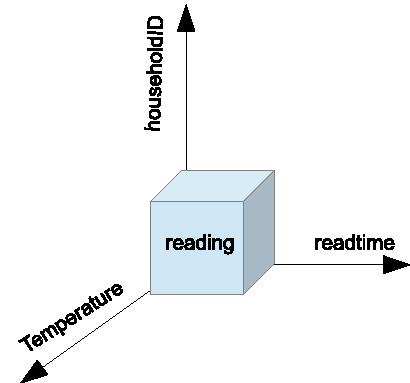
\includegraphics[width=0.4\textwidth]{images/scidbdatamodel}
\caption{Data model for storing ESSEX data}
\label{fig:essexdatamodel}
\end{figure}

%\section{Paper Reading}
%\begin{itemize}
%\item {\bf L.~Wang, L. Tanm  C.~Yu, and Z.~Wu. ``Study and Application of Non-Linear Time Series Prediction in Ground Source Heat Pump System". In {\em Proc. of CECNet}, pp. 3522--3525, 2012.}
%\end{itemize}


\medskip
\begin{thebibliography}{1}

\bibitem{ibmbenchmark}
Ten Million Meters Scalable to One Hundred Million Meters for Five Billion Daily Meter Readings. Sept. 2011.

\bibitem{yang}
J.~Yang, Y.~Zhai, D.~Xu, et al. ``SMO Algorithm applied in
time series model building and forecast". In {\em Proc. of ICMLC}, 2007:2395-2400, 2012.

\bibitem{scidb}
SciDB \url{http://www.scidb.org/} as of 2013-12-07.

\bibitem{scidbr}
SciDBR \url{https://github.com/Paradigm4/SciDBR} as of 2013-12-07.




\end{thebibliography}



\end{document}
